
\section{Design of the proposed solution}\label{ch:design}

This section describes the design of our proposal to integrate IoT constrained devices as part of the privacy preserving system P2ABCE. The ultimate goal is to enable constrained IoT devices to play the Idemix User role, interacting autonomously in order to authenticate and demonstrate their credential attributes to any Verifier in a privacy-preserving fashion, addressing the power and memory constrains many IoT devices face.

%We decided to use P2ABCE with the Idemix as its Engine, because it is officially supported by the Idemix Library, it has the most up-to-date implementation, as we saw in the state of the art, and adds capabilities to Idemix like the Presentation Policies, or interoperability with U-Prove, not available without the P2ABCE project.


% TODO sección de Requerimientos y objetivos
Our main goal is to make an IoT device capable to act as a User or Verifier in the P2ABCE architecture. For this, the device should be able to \textbf{communicate} with the Verifier or Prover with which it is interacting, manage the P2ABCE complex \textbf{XML schemas} transmitted, and perform the \textbf{cryptographic operations} required.

The communication between actors depends on each IoT scenario, it can be achieved with many existing standard solutions, e.g. an IP network, a Bluetooth M2M connection, RF communication, etc.

We also analysed how the P2ABCE architecture uses the logic of smart cards to gather the cryptographic operations independently from how the data is exchanged between P2ABCE actors.

Our real concerns are, on one side, parsing the XML data, based on the P2ABCE's XML schema, that specifies the data artifacts created and exchanged during the issuance, presentation, revocation and inspection of pABCs; and on the other side, the cryptographic operations, that involve the use of secret keys, stored privately in the IoT device.

%After the analysis done in the previous sections to the P2ABCE architecture, emphasizing that the logic of smart cards gathers the cryptographic operations independently from how the data is exchanged between P2ABCE actors.

Using the \textit{computation offloading} technique to our scenario, our design consists on implementing the smart card logic inside the IoT device, keeping safe our master key and credentials, and for the rest of the P2ABCE system, if the device can not run the complete Engine, it may delegate to a server running it, indicating how to send APDU Commands to the \textit{IoT smart card}.

Even in the case we were to implement all P2ABCE inside an IoT device, we would have to implement the support for software smart cards, to keep the secret inside the IoT device. Therefore, we can begin implementing the smart card logic inside the IoT device, and later, if the device resources admit it, other components of the P2ABCE project.


\hfil

Computation offloading is not a new technique for IoT environments. For example, to reduce the overhead of IPv6 we use 6LoWPAN to compress packets and use smaller address sizes. In order to communicate a 6LoWPAN with other networks, the IoT devices delegate on a proxy that can manage the 6LoWPAN and IPv6 stacks. In the scope of consumer devices, smart watches can install applications which delegate on the user's phone to accomplish performance demanding task. 
Therefore, the IoT device now has a \textbf{duality} in its functions, because it is the User that starts any interaction with other actors, and it is also the smart card that a P2ABCE server must ask for cryptographic operations. It can also be seen as a \textbf{double delegation}. The IoT device delegates on the external P2ABCE server to manage the protocol, and that P2ABCE server delegates on the IoT device, acting now as the smart card.

%TODO adaptar mejor a design
\subsection{Fundamentals on Zero-Knowledge Proofs}

% Ejemplo de DL problem
% Firma CL
% Mostrar al final la estructura de la mayoría de ZKP : commitment(s), challenge, response(s)

For a deep introduction to ZKPs, we recommend reading \textit{Fundamentals of Computer Security} \cite[Chapter 12]{book:856771}, but to show how one can indeed proof knowledge of a value, without revealing it, here we show the classic \textit{zero-knowledge proof of knowledge} based on the discrete logarithm problem, also known as Schnorr's identification scheme. Based on this discrete logarithm ZKP, Idemix then derives multiple ZK proofs of relations and properties of the values hidden.


Using the notation introduced by Camenisch and Stadler \cite{camenisch1997efficient}, the discrete logarithm ZKP can be written as 
\[ PK\{ (\alpha) : y = g^\alpha \}  \]
given a known group $G=\left\langle g \right\rangle $ of prime order $q$ and public value $y\in G$. The notation means: ``we know a secret value $\alpha$ such that $g^\alpha$ is $y$'', i.e. the discrete logarithm of $y$, $log_g y = \alpha$.


During the first step of the protocol, the prover chooses randomly a value $r_\alpha$, computes the \textit{commitment} $t := g^{t_\alpha}$ and sends $t$ to the verifier. 
Then, the verifier chooses another random exponent, the \textit{challenge} $c$, and sends it to the prover. 
Next, the prover computes the \textit{response} $s:=r-c\alpha\, mod\, q$ and sends it to the verifier.
Finnaly, the verifier checks whether or not $ t \overset{?}{=} g^{s_\alpha} y^c $ holds. The verifier never receives the secret value $\alpha$, and the verifier will not be able to compute it given $t$ and $s$.

\begin{figure}[bth]
	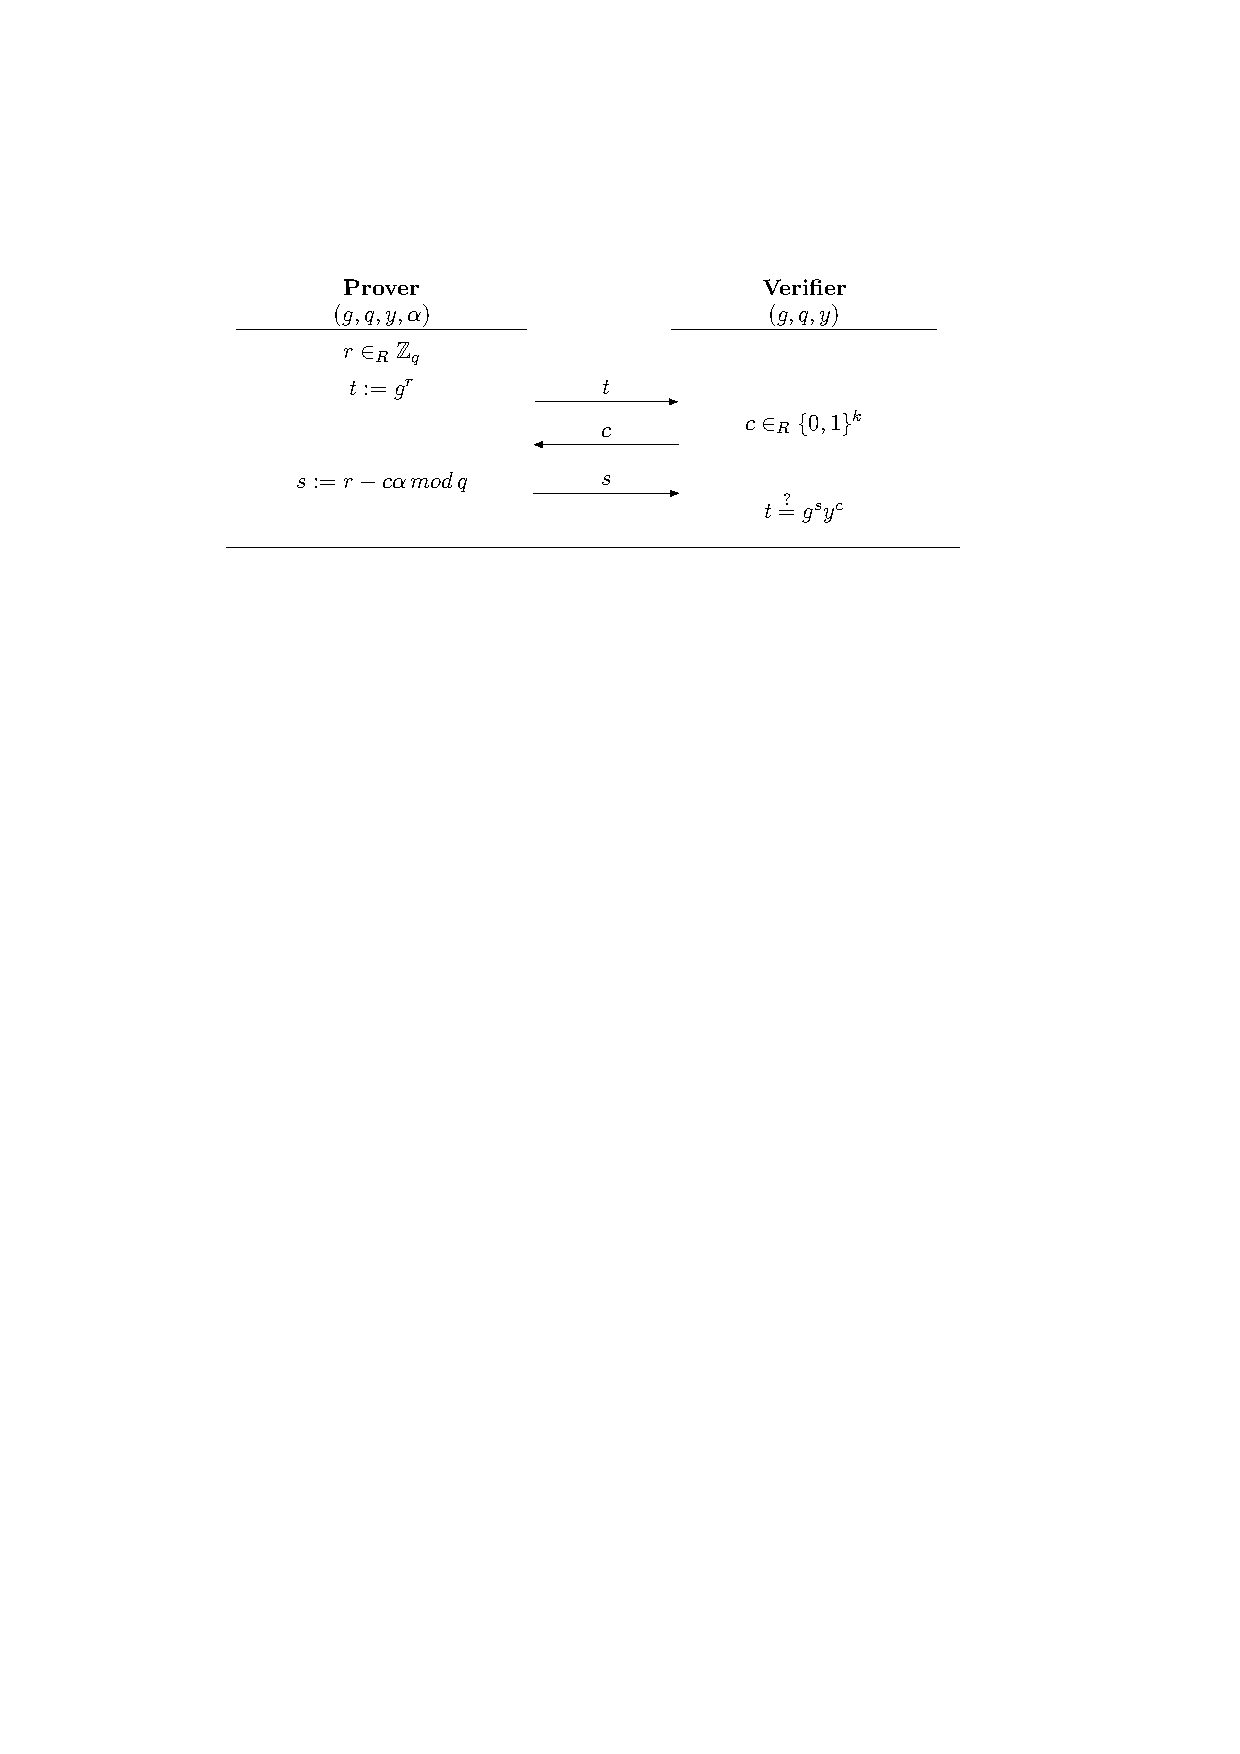
\includegraphics[width=\linewidth]{gfx/schnorr}
	\caption{$PK\{ (\alpha) : y = g^\alpha \}$ Schnorr's protocol. The prover knows $(g,q,y,\alpha)$ such that $g^\alpha=y$. The verifier knows $(g,q,y)$.}
	\label{fig:schnorr}
\end{figure}

We can see that the protocol works because $ g^{s_\alpha} y^c = g^{r_\alpha - c\alpha} (g^\alpha)^c =  g^{r_\alpha - c\alpha} g^{c\alpha} =
g^{r_\alpha - c\alpha + c\alpha} = g^{r_\alpha} = t $.

Going one step further, the Fiat-Shamir heuristic lets us replace the verifier challenge with a hash function $\mathcal{H}$, computing the challenge as $c:=\mathcal{H}(g\mid\mid y\mid \mid t\mid\mid n)$. The value $n$ is a random nonce generated by the verifier prior to this non-interactive ZKP. The nonce makes the verifier trust that the current ZKP is fresh and not a forgery from a previous ZKP.

In Idemix every ZKP follows the same scheme as shown in here. First, we have the \textit{commitment} \texttt{t}, next the \textit{challenge} \texttt{c} (computed with $\mathcal{H}$), and finally, the \textit{response} \texttt{s}. A prover can also achieve parallel ZKPs, she first computes the multiple \texttt{t}-values, next, she computes the same challenge \texttt{c} for every simultaneous ZKP, by combining all the information in one hash $\mathcal{H}$ call, and then she calculates all the \texttt{s}-values in parallel.

Therefore, to describe any proof being performed by the User, we can focus on the key steps of computing the \texttt{t}-values, challenge \texttt{c} and \texttt{s}-values, ignoring what specific mathematical operations are actually happening.

%\hfil
%%%
%Combining the ZKPs based on the discrete logarithm with the CL-signature over the credential attributes, one can achieve selective disclosure and other predicates over the attributes.
%%%

\subsection{System architecture}


\begin{figure*}[htb!]
	\centering
	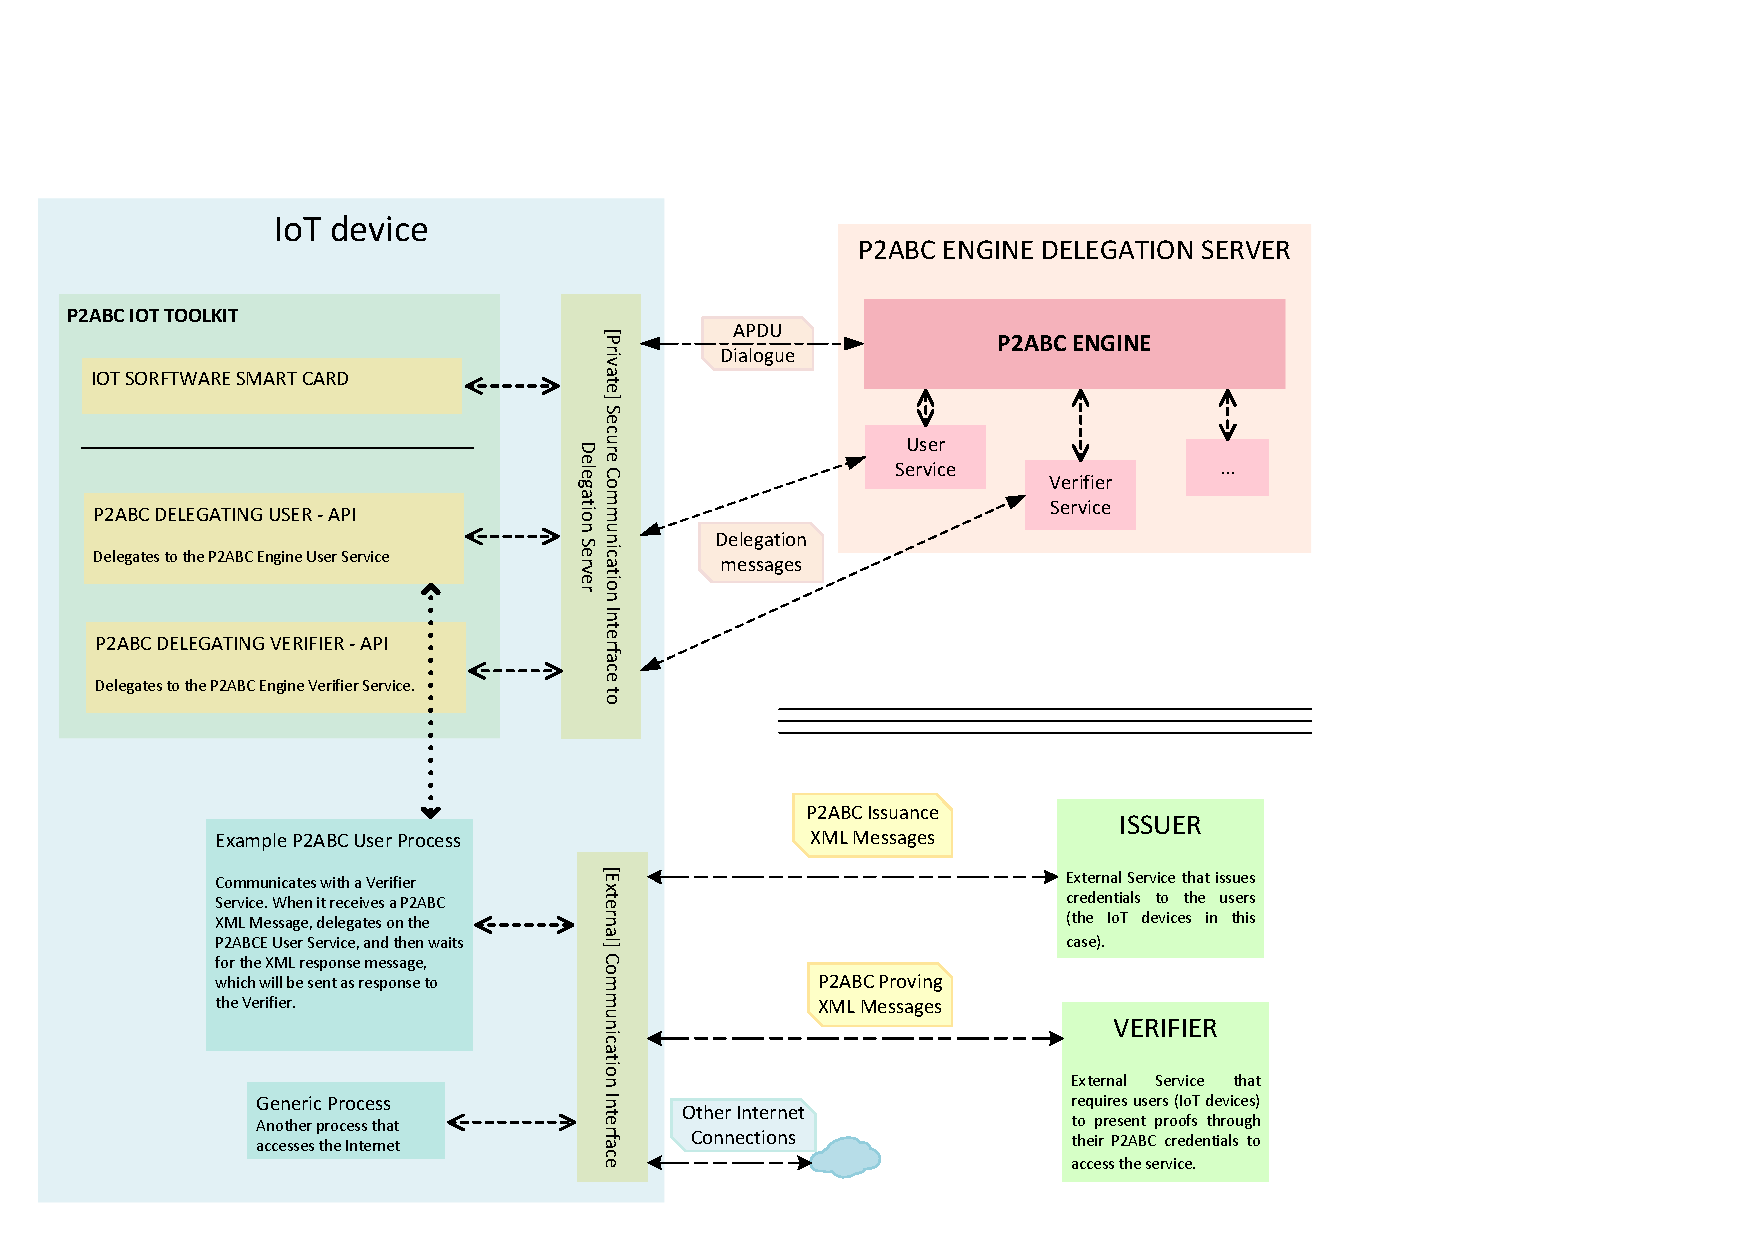
\includegraphics[width=0.7\textwidth]{gfx/P2ABCE-IoT-color}
	\caption{Proposed high level Architecture for integrating IoT devices in P2ABCE.}
	\label{fig:P2ABCE-IoT}
\end{figure*}

%\begin{figure}[bth]
%	\begin{center}
%		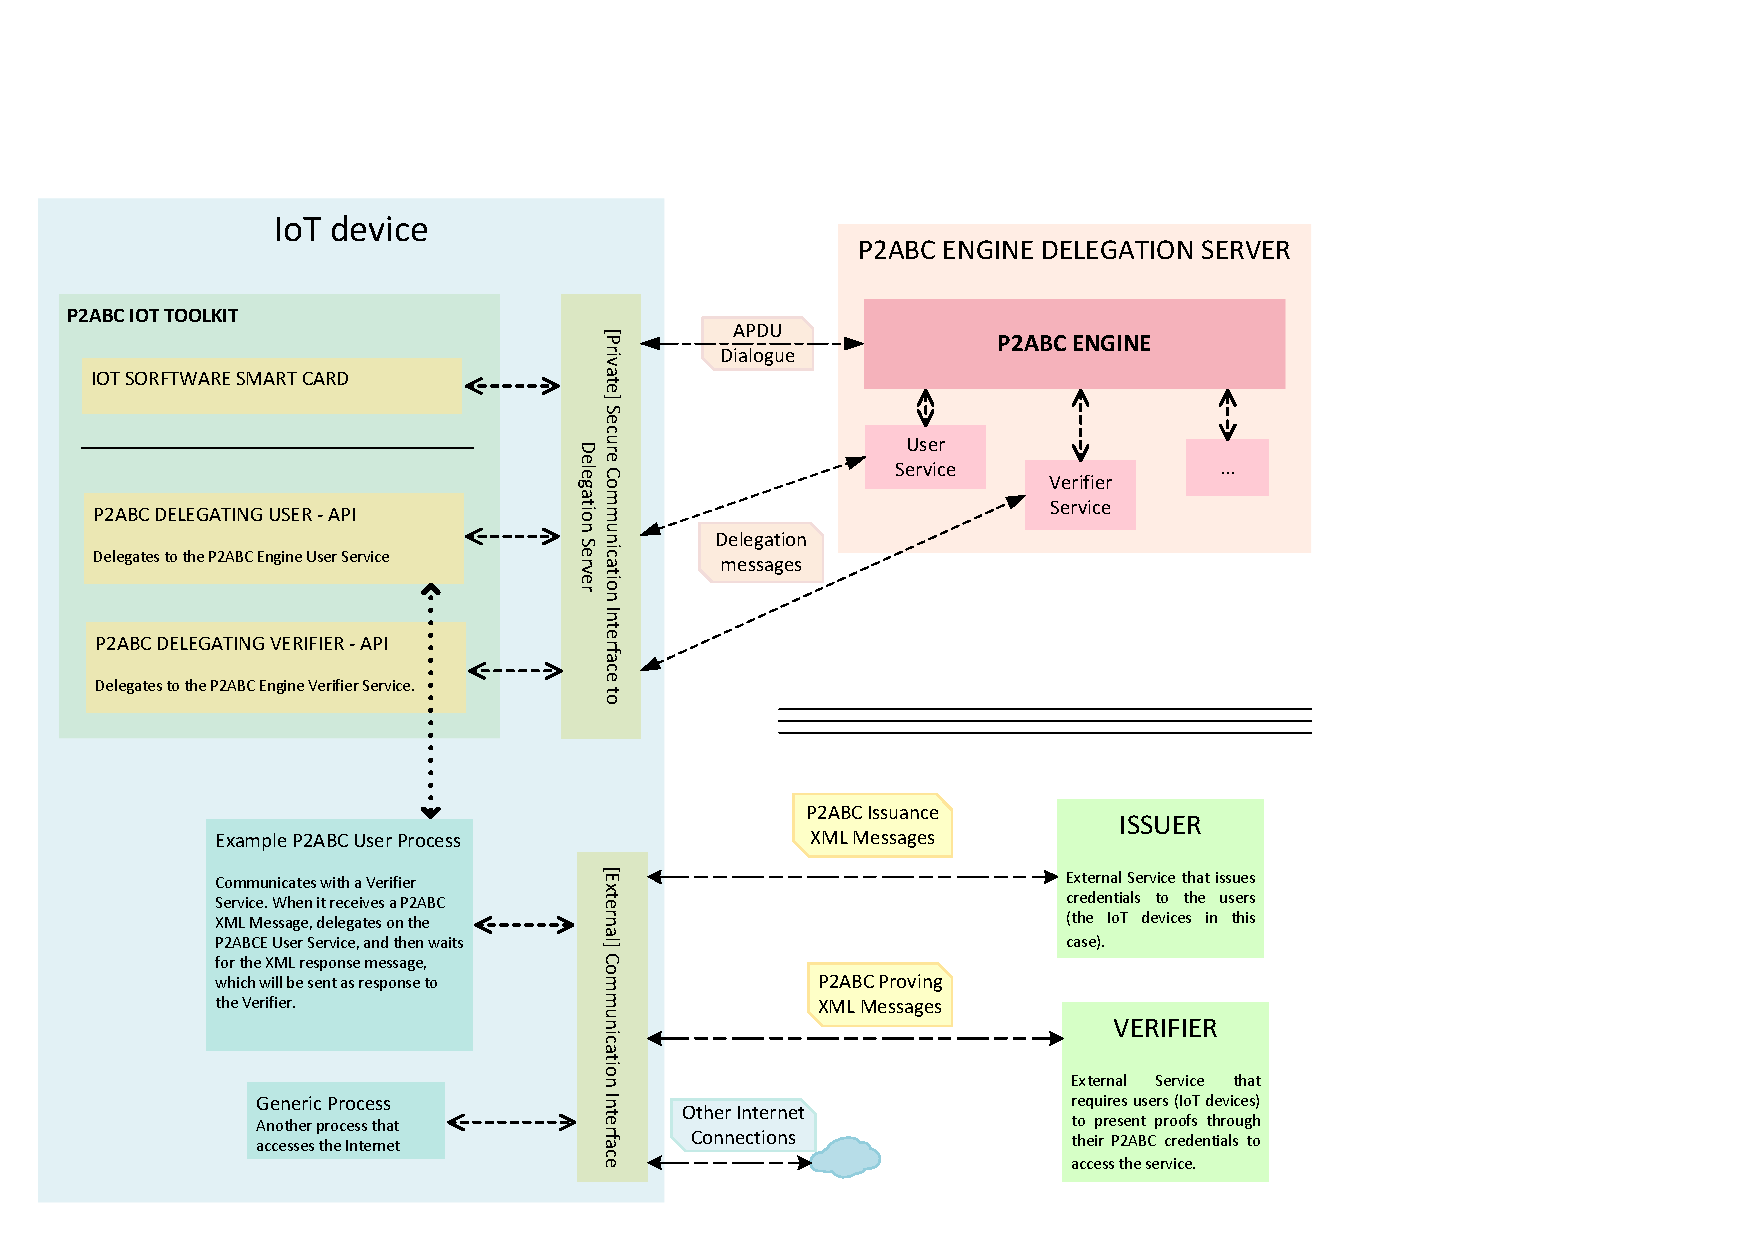
\includegraphics[width=\linewidth]{gfx/P2ABCE-IoT-color}
%	\end{center}
%	\caption{IoT in P2ABCE deployment diagram.}
%	\label{fig:P2ABCE-IoT-color}
%\end{figure}

\hfil


The system will be compounded by the IoT device, the P2ABCE delegation server and the third party P2ABCE actors:

\begin{itemize}
	
	\item \textbf{IoT device}
	
	\autoref{fig:P2ABCE-IoT} shows our proposed architecture, in which the IoT device is represented with two interfaces, physical or virtual. One allows external communications to other machines, including other P2ABCE actors. Through this interface, the P2ABCE XML messages are exchanged as in any other scenario. This lets an IoT device to interact with other actors without adaptations of the protocol. The other interface allows a secure communication with the delegation server. Both the delegation messages and the APDU Dialogue are transmitted over this interface, making it a point of attack, that we will talk about during the delegation process.
	
	The scheme also shows the \textit{P2ABCE IoT Toolkit}. This piece of software includes the \textit{IoT Smart Card}, and the P2ABCE API.
	
	The \textit{IoT Smart Card} is the implementation of a software smart card, listens for APDU Commands from the secure interface and stores securely the credentials and private keys within the device's memory.
	
	The P2ABCE API is an interface for other processes that wish to use the private-preserving environment of P2ABCE. It provides access to every operation available, hiding the delegation process to the server. In the future we could implement, for example, the Verification Service to run entirely in the IoT device, then the toolkit would conceal the transition from delegation to native execution.
	
	
	\item \textbf{P2ABCE actors}
	
	The possible roles in a P2ABC system are the Issuer, the User, the Verifier, the Revocation Authority and the Inspector, where these last two actors are optional. All of them use the P2ABCE XML schemas present in the specification to communicate to each other. Any third party actor that communicates with the IoT device will be unaware of the fact that the device is a constrained device that delegates on a P2ABCE server.
	
	\begin{figure}[bth]
		\begin{center}
			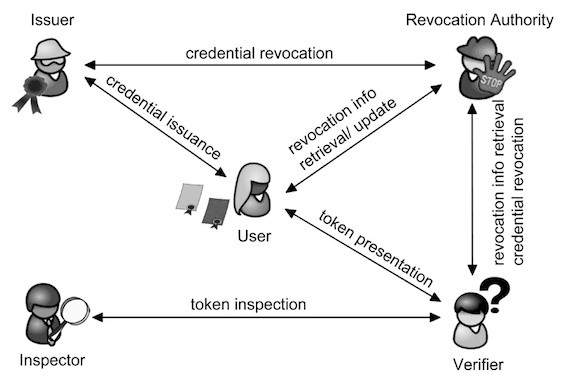
\includegraphics[width=0.8\linewidth]{gfx/actors.jpg}
		\end{center}
		\caption{Entities in a P2ABC System. Source: P2ABCE project.}
		\label{fig:actors}
	\end{figure}
	
	
	
	\item \textbf{P2ABCE Delegation Server}
	
	The machine in charge of receiving authorized IoT devices' commands to parse the XML files exchanged and orchestrate the cryptographic operations the IoT smart card must perform.
	
	
\end{itemize}

%\hfil
%
%\begin{flushleft}
%	\textbf{Delegation process}
%\end{flushleft}

\subsection{Delegation process}

In this section we describe the computation offloading carried out by the IoT device.  In \autoref{fig:DelegationProving} we show an example of the IoT acting as a User, carrying out a proving of a Presentation Policy to a third party Verifier.

\begin{enumerate}
	\item Communication with P2ABCE actor.
	
	The IoT device, acting as a User, starts an interaction with another actor, like an Issuer to obtain a signed credential, or a Verifier to demonstrate certain property of its attributes in a privacy-preserving way.
	
	\item Delegation to the P2ABCE Server.
	
	Depending on what role the IoT device is acting as, it will delegate to the corresponding service, e.g. User Service. The delegation message will include the XML data, and any parameter required to accomplish the task, like the information on how to communicate back with the IoT smart card.
	
	\item APDU Dialogue.
	
	The server may need to send APDU Commands to the \textit{IoT smart card} to read the credential information or perform cryptographic operations involving private keys, necessarily stored inside the IoT device.
	
	\item Server response.
	
	The server may return a status code indicating success, or an XML file if the third party actor requires an answer from the IoT device.
	
\end{enumerate}

\begin{figure}[bth]
	\begin{center}
		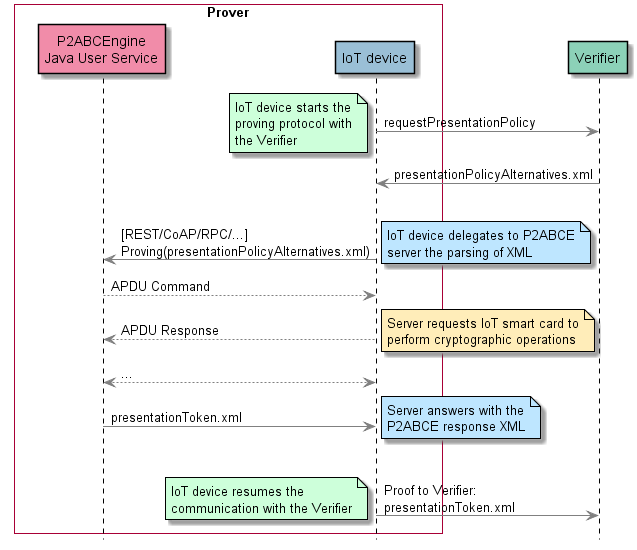
\includegraphics[width=\linewidth]{gfx/UML/provingDelegation}
	\end{center}
	\caption{Messages exchanged during the proving delegation.}
	\label{fig:DelegationProving}
\end{figure}

Transmissions over the \textit{Server-IoT} channel must be secured in order to avoid attacks like impersonating the P2ABCE delegation server, an attacker sending APDU Commands to the IoT smart card, or delegating as a device to the server but giving the parameters of another device, making the delegation server send the APDU Commands to a victim IoT smart card.


We could use a corporative PKI to issue certificates to the server and devices and configure policies for access control; design a challenge-response system combined with the smart card PIN, like a password and TOTP\footnote{Time-based One-time Password} in a 2FA\footnote{Two-factor authentication} login. We also could connect physically the delegation service through RS-232 serial to the IoT device, securing both physically as we would do with the IoT device on its own, isolating the delegation system from any network attack. % This last idea is an approximation to the Arduino Y\'un\footnote{\url{https://www.arduino.cc/en/Main/ArduinoBoardYun}}, a development board that integrates two microcontrollers, one a typical Arduino with very low resources, and another one running a fork of OpenWrt. The Arduino microcontroller can control the terminal of the more powerful one, using the serial pins as commented before.

As we can see, there are many state of the art solutions for all this threads, therefore, we can assume a secure channel without mentioning a specific solution, providing freedom to choose the most fitting one in a real deployment.

%%%%%%%%%%%%%

\hfil

Regarding the definition of the P2ABCE API, it is a work in progress, and in the meantime, we will work with the REST API currently available in the P2ABCE project to perform the delegation. Regarding the \textit{IoT Smart Card}, the P2ABCE project defines the APDU instructions with the corresponding format of the APDU Commands and Responses. In the next section we will explain the PoC for IoT based on these P2ABCE specifications.





%%%%%%%%%%%%%